\let\negmedspace\undefined
\let\negthickspace\undefined
\documentclass[journal]{IEEEtran}
\usepackage[a5paper, margin=10mm, onecolumn]{geometry}
%\usepackage{lmodern} % Ensure lmodern is loaded for pdflatex
\usepackage{tfrupee} % Include tfrupee package

\setlength{\headheight}{1cm} % Set the height of the header box
\setlength{\headsep}{0mm}     % Set the distance between the header box and the top of the text
\usepackage{multicol}
\usepackage{gvv-book}
\usepackage{gvv}
\usepackage{cite}
\usepackage{amsmath,amssymb,amsfonts,amsthm}
\usepackage{algorithmic}
\usepackage{graphicx}
\usepackage{textcomp}
\usepackage{xcolor}
\usepackage{txfonts}
\usepackage{listings}
\usepackage{enumitem}
\usepackage{mathtools}
\usepackage{gensymb}
\usepackage{comment}
\usepackage[breaklinks=true]{hyperref}
\usepackage{tkz-euclide} 
\usepackage{pgfplots}
\pgfplotsset{compat=1.18}
\usepackage{listings}
% \usepackage{gvv}                                        
\def\inputGnumericTable{}                                 
\usepackage[latin1]{inputenc}                                
\usepackage{color}                                            
\usepackage{array}                                            
\usepackage{longtable}                                       
\usepackage{calc}                                             
\usepackage{multirow}                                         
\usepackage{hhline}                                           
\usepackage{ifthen}                                           
\usepackage{lscape}
\usepackage{tikz}
% Marks the beginning of the document
\begin{document}
\bibliographystyle{IEEEtran}
\vspace{3cm}

\title{Solving differential equation\\NCERT-12.8.3.2}
\author{EE24BTECH11056 - S.Kavya Anvitha}
\maketitle
%\newpage
\bigskip

\renewcommand{\thefigure}{\theenumi}
\renewcommand{\thetable}{\theenumi}
\textbf{Question:}\\
Find the area between the curves $y = x$ and $y = x^2$.\\
\textbf{Exact Integral Solution:}\\
The point of intersection of the line with the parabola is $x_i=h+k_i m$,\\
where,$k_i$ is a constant and is calculated as follows:-
$$k_i=\frac{1}{m^\top Vm}\brak{-m^\top \brak{Vh+u}\pm \sqrt{\sbrak{m^\top \brak{Vh+u}}^2-g\brak{h}\brak{m^\top Vm}}}$$\\
\begin{align}
 V = \myvec{1 & 0\\0 & 0}\\
 f = 0\\
 u = -\myvec{0 \\ 2a} \text{here} \hspace{2mm} 4a = 1 \text{so} 2a = \frac{1}{2}\\
 u = \myvec{0\\-\frac{1}{2}}
 m = \myvec{1\\1}
\end{align}
Substituting the input parameters in $k_i$,\\
we get: $x_1 = \myvec{0\\0}$ and $x_2 = \myvec{1\\1}$
The area between the curves can be found using the definite integral:
\begin{align}
    A = \int_{0}^{1} (x - x^2) \, dx
\end{align}
 Calculating the integral term by term:
\begin{align}
    A = \left[ \frac{x^2}{2} - \frac{x^3}{3} \right]_0^1
\end{align}
\begin{align}
    = \frac{1}{2} - \frac{1}{3} = \frac{1}{6} \approx 0.1667
\end{align}
\textbf{By using trapezoidal rule:}\\
The area between the curves 
$y=x$ and $y=x^2$ can be calculated using the trapezoidal rule by integrating the difference between the curves. The area can be expressed as:
\begin{align}
    A = \int_{a}^{b} f(x) \, dx
\end{align}
where the curves intersect at $x=0$ and $x=1$\\
\textbf{Trapezoidal rule formula:}\\
The trapezoidal rule approximates the integral using the formula:\\
\begin{align}
    A \approx \frac{h}{2}\sbrak{f(x_0)+2\sum_{i=1}^{n-1} f(x_i) + f(n)}
\end{align}
where:\\
\begin{enumerate}
   \item $h=\frac{b-a}{n}$ is the width of each subinterval.
   \item $f(x) = x-x^2$.
   \item $a=0,b=1$.
   \item $n$ is the number of subintervals.
\end{enumerate}
Taking trapezoid shaped strips of small area and adding them all up.. Say we have to
find the area of $y(x)$ from $x=x_0$ to $x = x_n$,discretize points on the x axis $x_0,x_1,x_2,...,x_n$ such that they are equally spaced with step-size h.Sum of all trapezoidal areas is given by,
\begin{align}
    A = \frac{1}{2}h\brak{y(x_1)+y(x_0)}+\frac{1}{2}h\brak{y(x_2)+y(x_1)}+\frac{1}{2}h\brak{y(x_3)+y(x_2)}+\dots+\frac{1}{2}h\brak{y(x_n)+y(x_{n-1)}}\\
    = h\sbrak{\frac{1}{2}\brak{y(x_0)+y(x_n)}+y(x_1)+y(x_2)+\dots+y(x_{n-1})}
\end{align}
Let $A(x_n)$ be the area enclosed by the curve $y(x)$ from $x=x_0$ to $x=x_n$
\begin{align}
    A(x_{n}+h) = A(x_n) + \frac{1}{2}h\sbrak{y(x_{n}+h)+y(x_n)}
\end{align}
we can repeat this till we get a required area
\begin{align}
    A_{n+1} = A_n + \frac{1}{2}h\sbrak{y_{n+1}+y_n}
\end{align}
We can write $y_{n+1}$ in terms of $y_n$ as $y_{n+1} = y_n + h\cdot y^{\prime}_n$
Substituting in the equation we get:
\begin{align}
    A_{n+1} = A_n +\frac{1}{2}h\sbrak{\brak{y_n+h\cdot y^{\prime}_n}+y_n}\\
    A_{n+1} = A_n + hy_n + \frac{1}{2}h^2y^{\prime}_n\\
    x_{n+1} = x_n + h
\end{align}
In the given question $y_n = x_n - x^2_n$ and $y^{\prime}_n = 1-2x_n$\\
General difference equation will be given by:
\begin{align}
    A_{n+1} = A_n + hy_n + \frac{1}{2}h^2y^{\prime}_n\\
    A_{n+1} = A_n + h\brak{x_n - x^2_n} + \frac{1}{2}h^2\brak{1-2x_n}\\
    A_{n+1} = A_n - hx^2_n + \brak{h-h^2}x_n + \frac{h^2}{2}\\
    x_{n+1} = x_n + h
\end{align}
Using \brak{n = 4} subintervals as an example:
\begin{align}
    h = \frac{1 - 0}{4} = 0.25
\end{align}
The points are: 
\begin{align}
    x_0 = 0, \quad x_1 = 0.25, \quad x_2 = 0.5, \quad x_3 = 0.75, \quad x_4 = 1
\end{align}
Function values:
\begin{align}
    f(0) = 0, \quad f(0.25) = 0.1875, \quad f(0.5) = 0.25, \quad f(0.75) = 0.1875, \quad f(1) = 0
\end{align}
Applying the trapezoidal rule formula:
\begin{align}
    A \approx \frac{0.25}{2} \left[0 + 2(0.1875 + 0.25 + 0.1875) + 0\right]
\end{align}
\begin{align}
    A \approx \frac{0.25}{2} \times 1.25 = 0.15625
\end{align}

\textbf{Comparison with Exact Area:}\\
The exact area calculated earlier was:
\begin{align}
    A_{\text{exact}} = \frac{1}{6} \approx 0.1667
\end{align}
The area calculated using the trapezoidal rule with \brak{n=4} is:
\begin{align}
    A_{\text{trapezoidal}} \approx 0.15625
\end{align}
The approximation improves as the number of subintervals increases. Therefore, the trapezoidal rule provides a close estimate of the integral as the step size decreases.
\begin{figure}[h!]
   \centering
   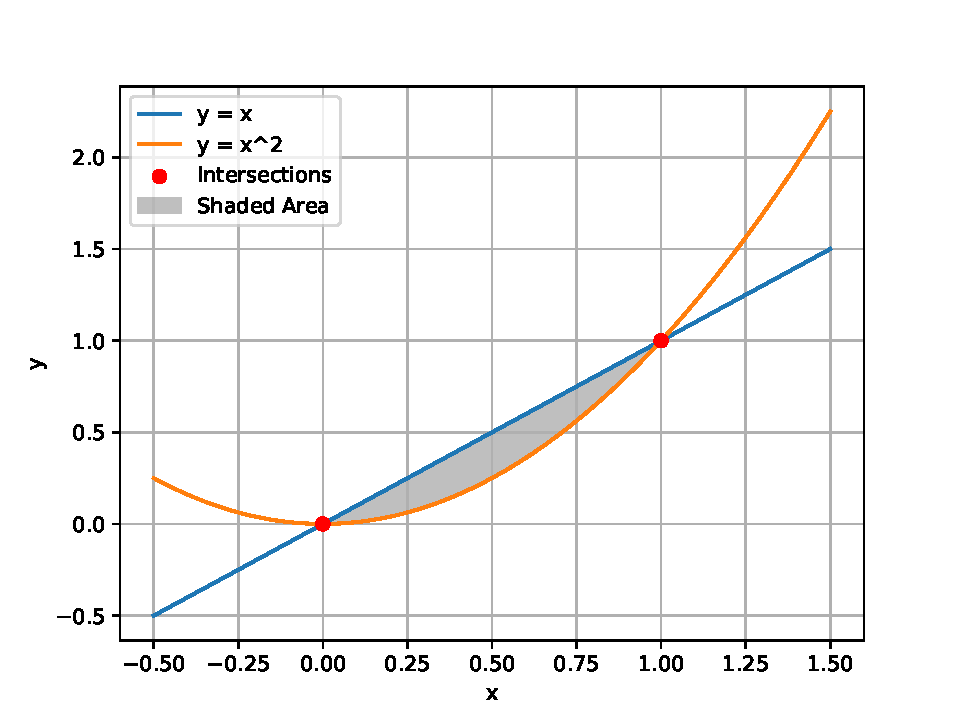
\includegraphics[width=\columnwidth]{figs/fig.pdf}
\end{figure}
\end{document}

